
%%%%%%%%%%%%%%%%%%%%%%%%%%%%%%%%%%%%%%%%%%%%%%%%%%%%%%%%%%%%%%%%%%%%%%%%%%%%%%%%%%%%%%%
\section{ Método de Newton para funções $h(x)$: $\mathbb{R}$ $\rightarrow$ $\mathbb{R}$ }

\begin{theorem}[Solução iterativa]\label{theo:rootshx}
~\\
\begin{minipage}{0.20\textwidth}
\centering
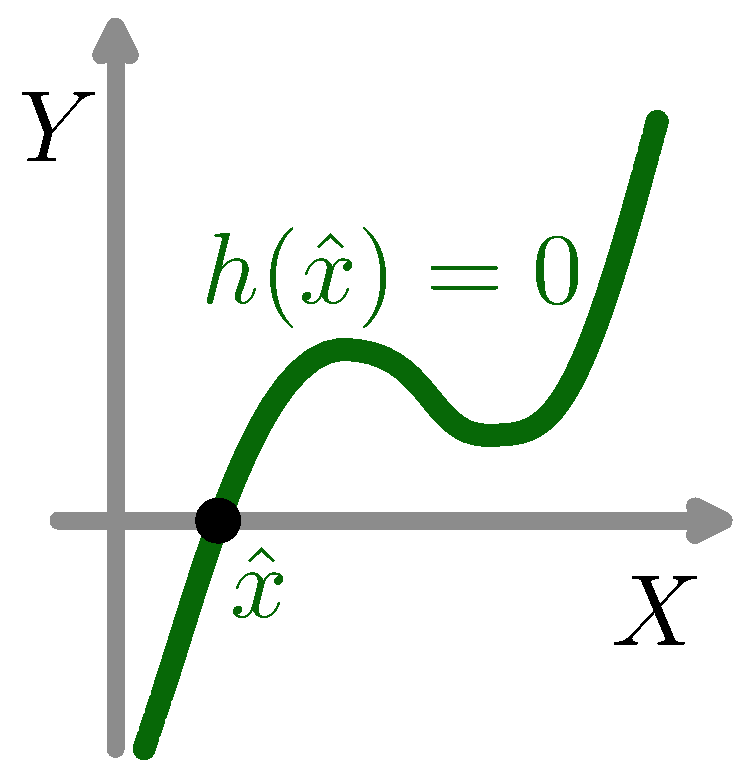
\includegraphics[width=0.9\linewidth]{chapters/roots/roots1.eps} 
\end{minipage}
\begin{minipage}{0.8\textwidth}
Dados
um escalar $\delta \in \mathbb{R}_+$, 
um escalar $x \in \mathbb{R}$, 
uma função $h:\mathbb{R} \rightarrow \mathbb{R}$, e 
conhecida a validade da Eq. (\ref{eq:rootshx1}),
\begin{equation}\label{eq:rootshx1}
0=h(x);
\end{equation}
se desejarmos ter o valor $x=\hat{x}$ que cumpra a Eq. (\ref{eq:rootshx1}),
podemos usar iterativamente a Eq. (\ref{eq:rootshx2}),
na qual $h'(x)\equiv \frac{d h(x)}{d x}$,
\end{minipage}

\begin{equation}\label{eq:rootshx2}
x_{k} \leftarrow x_{k-1}-\frac{ h(x_{k-1})}{h'(x_{k-1})}.
\end{equation}
Assim, $\hat{x}$ pode ser achado\footnote{A 
demonstração pode ser vista na Prova \ref{proof:theo:rootshx}.} 
iniciando a Eq. (\ref{eq:rootshx2}) desde um 
$x_{0}$ qualquer, realizando cálculos $x_{k}$ iterativamente  
até\footnote{Sendo $\delta$ um valor pequeno próximo a zero.} que $||h(x_k)||<\delta$,
nesse caso se declara que $\hat{x}=x_k$.

\textbf{Considerações:}
\begin{itemize} 
\item Se $h'(x_{k-1})\approx 0$, então estamos perto de um ponto de inflexão 
(máximo, mínimo ou ponto de sela) em $x_{k-1}$. Nesses pontos a Eq. (\ref{eq:rootshx2}): 
\begin{itemize}
\item Diverge quando se cumpre que $h(x_{k-1})\neq 0$, ou
\item Converge\footnote{A demonstração pode ser vista na Prova \ref{proof:theo:cont:rootshx}.} 
se $h(x_{k-1}) = 0$ e se verifica que $h(x)$ pode ser representado 
mediante uma \hyperref[def:taylor]{\textbf{série de Taylor}} ao redor de $x_{k-1}$, 
 pois indica que $\lim_{x\rightarrow x_{k-1}}  h(x)/h'(x)$ é finito.
\end{itemize}
\item Uma sugestão do procedimento para a busca de uma raiz pode ser vista no diagrama de fluxo
mostrado na Figura \ref{fig:fluxorhx1}. 
\end{itemize}
\end{theorem}

\begin{figure}[!h]
     \centering
         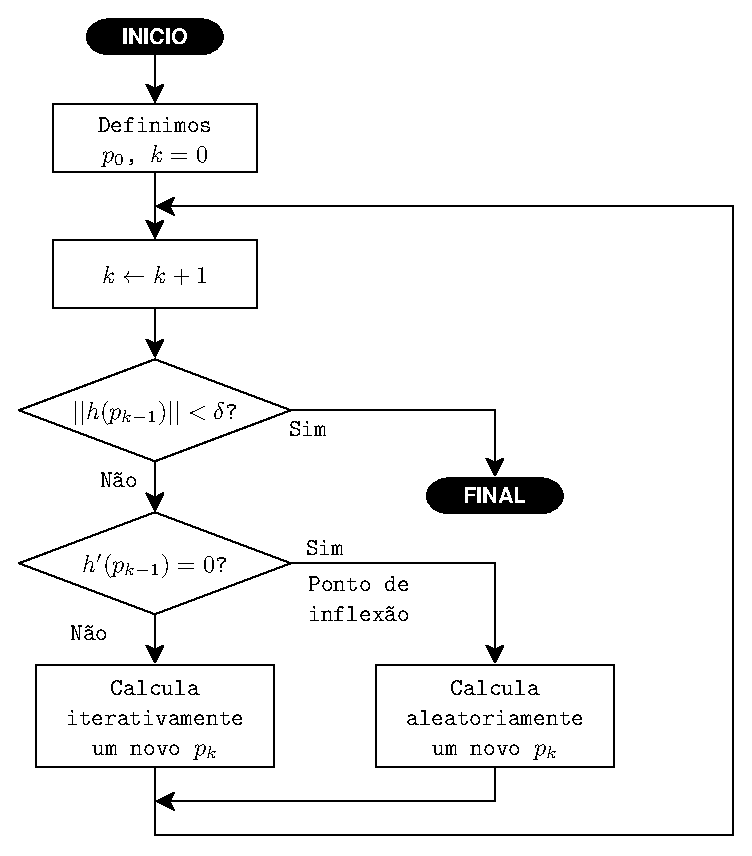
\includegraphics[width=0.75\textwidth]{chapters/roots/fluxo1.eps}
        \caption{Diagrama de fluxo da solução iterativa para achar uma raiz, seguindo o teorema \ref{theo:rootshx}.}
        \label{fig:fluxorhx1}
\end{figure}

\newpage
%%%%%%%%%%%%%%%%%%%%%%%%%%%%%%%%%%%%%%%%%%%%%%%%%%%%%%%%%%%%%%%%%%%%%%%%%%%%%%%%
\subsection{Exemplos de busca de raízes pelo método de Newton}


\begin{example}\label{ex:rootshx1}
Conhecida uma função $h(x)=x(x^2-1)+1$, e um escalar $\delta=10^{-3}$;
usando o Teorema \ref{theo:rootshx}, 
achar um valor $x=\hat{x}$ que cumpra $||h(x)||<\delta$.
Podemos ver as respostas a esse exemplo na Solução \ref{sol:rootshx1} e \ref{sol:rootshx2}.
\end{example}
\begin{SolutionT}[Relativa ao Exemplo \ref{ex:rootshx1} (Diverge):]\label{sol:rootshx1}
 A Fig. \ref{fig:rootsNcasesa} nos mostra o processo de busca das raízes de $h(x)$. 
A busca inicia em $x_0=-0.3$, 
todos os valores $x_{k}$ podem ser vistos na
Tabela \ref{tab:rootsNcases1}. 
Neste caso, a busca iterativa indicada pela Eq. (\ref{eq:rootshx2}) 
diverge para valores próximos a $x_m=\frac{\sqrt{3}}{3}\approx 0.57735$,
que é um mínimo local de $h(x)$; quer dizer, $h'(x_m)\approx 0$ e $h(x_m)\neq 0$.
É fácil de observar que neste caso se produz 
uma espécie de efeito sanfona, no qual $x_{k}$ se aproxima ao mínimo local em $h(x)$, e quando 
está próximo desse valor, a busca volta a divergir a um ponto medianamente distante.
\end{SolutionT}

\begin{figure}[!h]
    \centering
    \begin{subfigure}[b]{0.49\textwidth}
        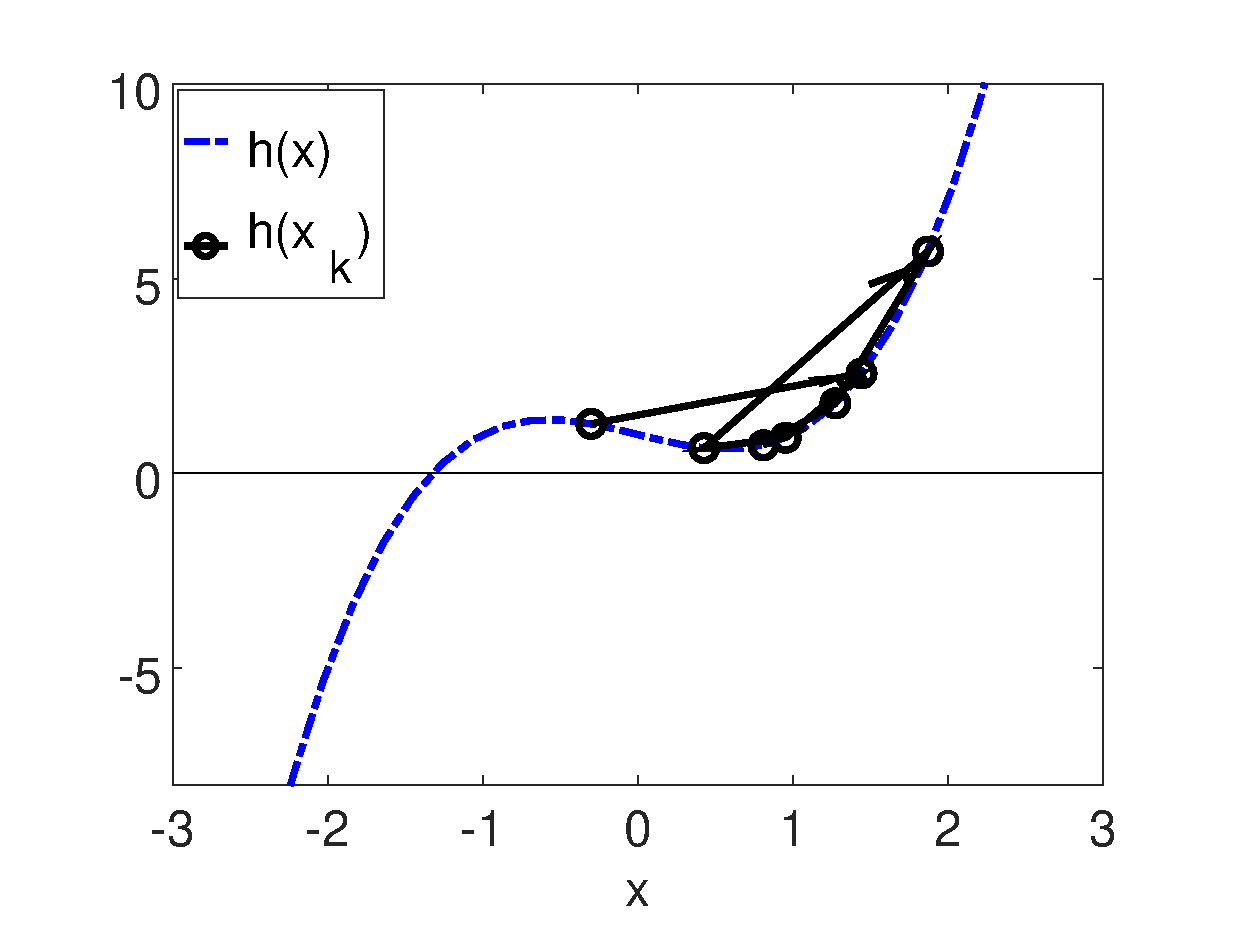
\includegraphics[width=\textwidth]{chapters/roots/mfiles/hx/minimizando_hx_1.eps}
        \caption{As iterações divergem ao redor da amostra $x_m$ em que $h'(x_m)\approx 0$ e $h(x_m)\neq 0$.}
        \label{fig:rootsNcasesa}
    \end{subfigure}
    ~ %add desired spacing between images, e. g. ~, \quad, \qquad, \hfill etc. 
      %(or a blank line to force the subfigure onto a new line)
    \begin{subfigure}[b]{0.49\textwidth}
        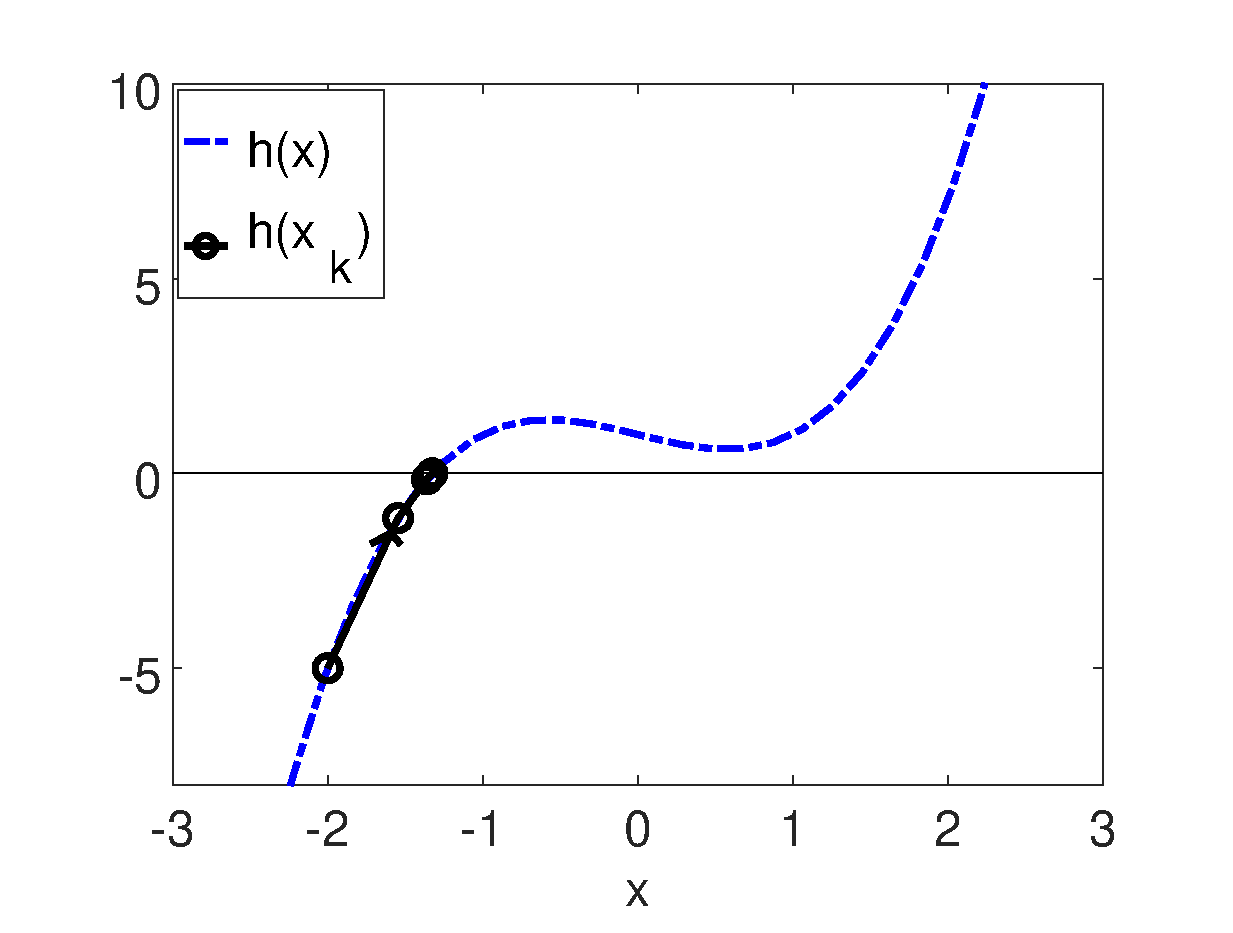
\includegraphics[width=\textwidth]{chapters/roots/mfiles/hx/minimizando_hx_2.eps}
        \caption{As iterações convergem em $\hat{x}$, no qual $h(\hat{x})\approx 0$ e $h'(x_m)\neq 0$.}
        \label{fig:rootsNcasesb}
    \end{subfigure}
    \caption{Comportamento da busca iterativa do Exemplo \ref{ex:rootshx1}}
    \label{fig:rootsNcases}
\end{figure}

\begin{table}[!h]
\centering
\begin{tabular}{|l|l|l|l|l|l|l|l|}
\hline
$k$      & 0 & 1 & 2 & 3 & 4 & 5 & 6\\ \hline
$x_k$    & -0.30000 & 1.44384 & 0.95543 & 0.42813 & 1.87298 & 1.27476 & 0.81109 \\ \hline
$||h(x_k)||$ & 1.27300 & 2.56607 & 0.91673 & 0.65034 & 5.69758 & 1.79676 & 0.72250 \\ \hline
\end{tabular}
\caption{Resposta iterativa do Exemplo \ref{ex:rootshx1}.}
\label{tab:rootsNcases1}
\end{table}

\begin{SolutionT}[Relativa ao Exemplo \ref{ex:rootshx1} (Converge):]\label{sol:rootshx2}
A Fig. \ref{fig:rootsNcasesb} nos mostra o processo de busca de uma raiz de $h(x)$. 
A busca inicia em $x_0=-2.0$,
 todos os valores $x_{k}$ podem ser vistos na Tabela \ref{tab:rootsNcases2}. 
Neste caso, a busca iterativa indicada pela Eq. (\ref{eq:rootshx2}) converge 
em $x_4\approx 0$ com $||h(x_4)||<\delta$ que corresponde a uma raiz de $h(x)$.
\end{SolutionT}

\begin{table}[!h]
\centering
\begin{tabular}{|l|l|l|l|l|l|}
\hline
$k$      & 0 & 1 & 2 & 3 & 4 \\ \hline
$x_k$    & -2.0000 & -1.5455 & -1.3596 & -1.3258 & -1.3247 \\ \hline
$||h(x_k)||$ & 5.0000 &  1.1458 & 1.5370e-01 & 4.6249e-03 & 4.6577e-06 \\ \hline
\end{tabular}
\caption{Resposta iterativa do Exemplo \ref{ex:rootshx1}.}
\label{tab:rootsNcases2}
\end{table}

\begin{example}\label{ex:rootshx2}
Conhecida uma função $h(x)=x(x^2-1)+2\frac{\sqrt{3}}{9}$ e um escalar $\delta=2~10^{-5}$;
usando o Teorema \ref{theo:rootshx},
achar o valor $x=\hat{x}$ que cumpra $||h(x)||<\delta$.
Podemos ver a resposta a este exemplo na Solução \ref{sol:rootshx3}.
\end{example}

\begin{SolutionT}[Relativa ao Exemplo \ref{ex:rootshx2} (Converge):]\label{sol:rootshx3}
A Fig. \ref{fig:rootsNcasesc} nos mostra o processo de busca de uma raiz de $h(x)$. 
A busca inicia em $x_0=-0.3$,
 todos os valores $x_{k}$ podem ser vistos na Tabela \ref{tab:rootsNcases3}. 
Neste caso, a busca iterativa indicada pela Eq. (\ref{eq:rootshx2}) converge 
em $x_4\approx 0$ com $||h(x_4)||<\delta$ que corresponde a uma raiz de $h(x)$.
Analiticamente podemos verificar que uma raiz pode ser achada em $x_m=\frac{\sqrt{3}}{3}\approx 0.57735$.
\end{SolutionT}

\begin{table}[!h]
\centering
\begin{tabular}{|l|l|l|l|l|l|}
\hline
$k$      & 0 & 1 & 2 & 3 & 4 \\ \hline
$x_k$    & -0.30000 & 0.60123 & 0.58937 & 0.58338 & 0.58037 \\ \hline
$||h(x_k)||$ & 6.5790e-01 & 1.0016e-03 & 2.5207e-04 & 6.3234e-05 & 1.5836e-05 \\ \hline
\end{tabular}
\caption{Resposta iterativa do Exemplo \ref{ex:rootshx1}.}
\label{tab:rootsNcases3}
\end{table}

    \begin{figure}[!h]
        \centering
        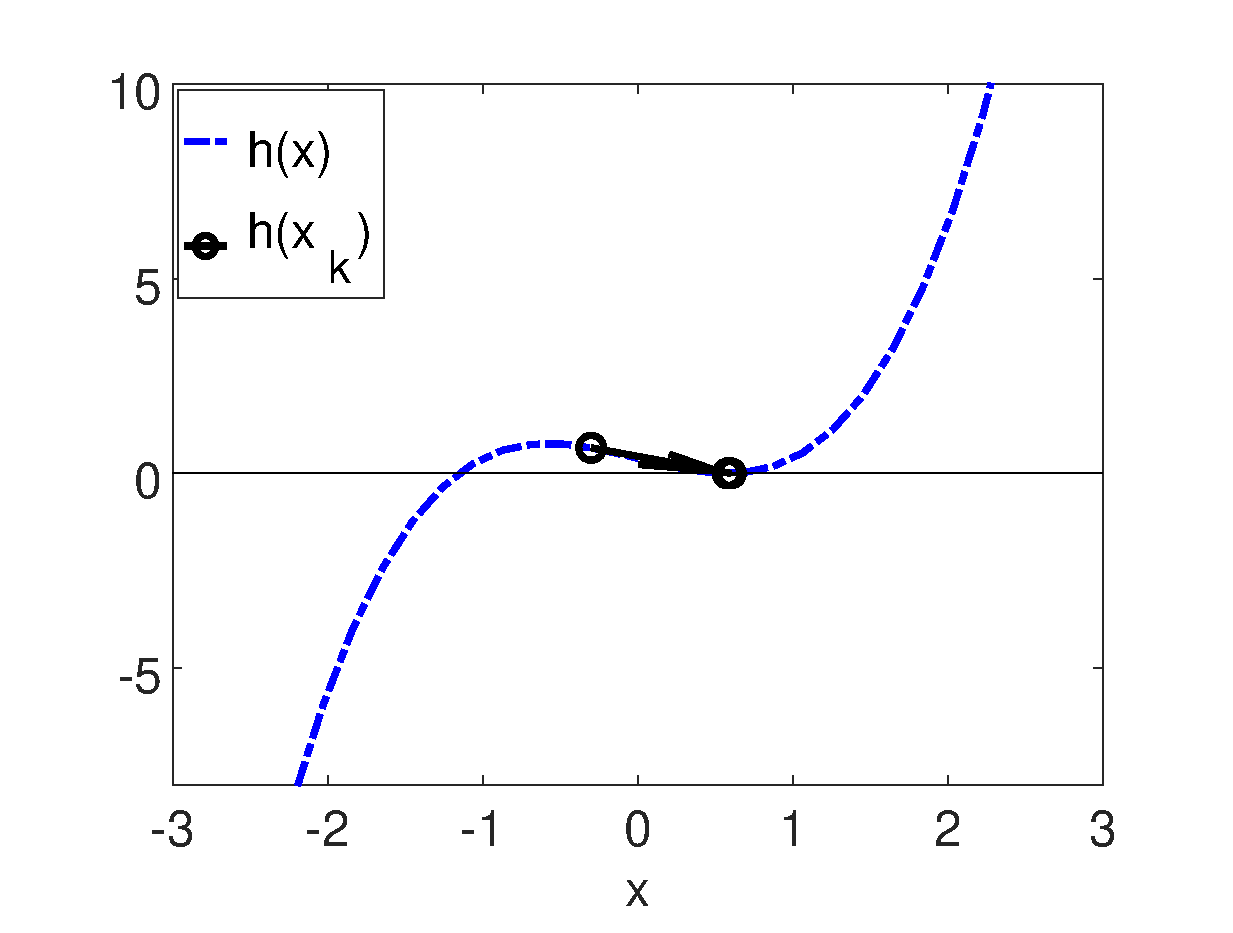
\includegraphics[width=0.49\textwidth]{chapters/roots/mfiles/hx2/minimizando_hx_1.eps}
        \caption{Resposta iterativa do Exemplo \ref{ex:rootshx2}, no qual $h'(x_m)\approx 0$ e $h(x_m)\approx 0$.}
        \label{fig:rootsNcasesc}
    \end{figure}

